\documentclass[11pt,a4paper]{article}
\usepackage{CJKutf8}

%\usepackage[T1]{fontenc}
\usepackage[utf8]{inputenc}
\usepackage{fancyhdr}

\usepackage{amsmath} \usepackage{balance} \usepackage{setspace}
\usepackage[title,titletoc,toc]{appendix} \usepackage{minted} \usepackage{url}
\usepackage{graphicx} \usepackage{wrapfig} \usepackage{subcaption}
\graphicspath{ {images/} }
% \usepackage[backend=biber, style=phys,]{biblatex}
\usepackage{tabu}
\usepackage[figurewithin=section,compatibility=false,justification=justified,listformat=simple,format=plain,labelformat=simple,labelsep=period]{caption}
\usepackage[top=1.4in,bottom=1.6in,left=1.in,right=1in]{geometry}
\usepackage{indentfirst}
% \addbibresource{elex.bib}

\usepackage{wrapfig}
\setlength{\parindent}{22pt} 
\setlength{\parskip}{.5em} 
\usepackage{hyperref}
\usepackage{xcolor}
\hypersetup{
	colorlinks,
	linkcolor={red!50!black},
	citecolor={blue!50!black},
	urlcolor={blue!80!black}
}


\renewcommand{\abstractname}{摘要} 
\renewcommand{\figurename}{图}
\renewcommand{\tablename}{表} 
\title{近代物理实验(I):光泵磁共振}

\author{胡乃超$^1$ \hspace{1cm}  金谷柳新$^2$\\
\footnotesize{ $^1$ 物理科学与工程技术学院, 物理学系$2013$级, $12309011$} \\
\footnotesize{ $^2$ 物理科学与工程技术学院, 物理学系$2013$级, $13345012$}}
 
% \author{金谷柳新$^1$ \hspace{1cm}  胡乃超$^2$\\
% \footnotesize{ $^1$ 物理科学与工程技术学院, 物理学系$2013$级, $13345012$} \\
% \footnotesize{ $^2$ 物理科学与工程技术学院, 物理学系$2013$级, $12309011$}}
  
\date{}

\makeatletter\@addtoreset{section}{part}\makeatother%

\begin{document}
\begin{spacing}{1.3}
\begin{CJK*}{UTF8}{gbsn}
\maketitle
    %\begin{abstract}
    %OMG 图终于正常了我好感动。XD
    %  啦啦啦啦啦啦啦啦啦啦啦啦啦啦啦啦啦啦啦啦啦啦啦啦啦啦啦啦啦啦啦啦啦啦啦啦啦啦啦啦啦啦啦啦啦啦啦啦啦啦啦
    %  啦啦啦啦啦啦啦啦啦啦啦啦啦啦啦啦啦啦啦啦啦啦啦啦啦啦啦啦啦
    %  啦啦啦啦啦啦啦啦啦啦啦啦啦啦啦啦啦啦啦啦啦啦啦啦啦啦啦啦啦啦啦啦啦啦啦啦啦啦啦啦
    %  啦啦啦啦啦啦啦啦啦啦啦啦啦啦啦啦啦啦啦啦啦啦啦啦啦啦啦啦啦啦啦啦啦啦啦啦啦啦啦啦
    %  啦啦啦啦啦啦啦啦啦啦啦啦啦啦啦啦啦啦啦啦啦啦啦啦啦啦啦啦啦啦啦啦啦啦啦啦啦啦啦啦\par
    %\textbf{关键词:}
    %\end{abstract}    
\section{引言}
光泵磁共振是把光抽运、磁共振和光探测技术有
机地结合起来以研究气态原子精细结构和超精细结构
的一种实验技术。
光泵磁共振是把光抽运、磁共振和光探测技术有
机地结合起来以研究气态原子精细结构和超精细结构
的一种实验技术 。
该技术既保存了磁共振高分辨的特点,同时又将
测量灵敏度提高了几个数量级,是研究原子、分子高
激发态的精密测量的有力工具,因此在激光物理、量
子频标、弱磁场探测等方面都有重要应用价值。
\section{实验目的}
\begin{enumerate}
\item 	熟悉光抽运效应和光磁共振的基本原理。
\item   加深对原子超精细结构的理解,测定铷原子超精细结构塞曼子能级的朗德$g_F$因子。
\end{enumerate}

\section{实验原理}
\subsection{铷($Rb$)原子基态和最低激发态能级}
 本实验的研究对象为气态自由铷($Rb$)原子,天然铷有两种同位素:$^{85}Rb$和$^{87}Rb$(分占$72.15\%$和$27.85\%$)。
 实验选用天然铷样品,即可在一个样品中观测到两种原子的超精细结构塞曼子能级跃迁的磁共振信号,
 又能更好的学习复杂现象分析的实验技能。\par
 铷是碱金属原子,在外壳层只有一个电子。其价电子处于第5壳层,即主量子数$n=5$;主量子数为$n$的电子,
 其轨道量子数$L=0,1,2,\ldots,n-1,n$,基态的$L=0$,最低激发态的$L=1$;电子具有自旋,电子自旋量子数$S=1/2$。
 由于电子自旋角动量与轨道角动量相互作用(即$LS$耦合),电子总角动量的量子数$J=L+S,L+S-1,\ldots,|L-S|$。
 对铷原子基态$L=0,S=1/2$故$J=1/2$,标记为$5^2S_{1/2}$;其最低激发$L=1,S=1/2$故$J=1/2$和$J=3/2$,
 分别标记为$5^2P_{1/2}$和$5^2P_{3/2}$双重态。他们是电子自旋角动量与轨道角动量耦合而产生的精细结构。
 $5^2P_{1/2} \to 5^2S_{1/2}$跃迁产生波长为794.8nm的$D_1$谱线,$5^2P_{3/2} \to 5^2S_{1/2}$跃迁产生波长
 $780.0mm$的$D_2$ 谱线。这两条谱线是铷原子主线系的第一条双线,也是铷灯光谱中最强谱线。\par
原子价电子在上述$L-S$耦合中,总角动量$P_J$与原子的电子总磁矩$\mu_J$ 的关系为
\begin{eqnarray} \label{2-6-1}
  \mu_J=-g_j\frac{e}{2m}P_J,
\end{eqnarray}
\begin{eqnarray} \label{2-6-2}
  g_J=1+\frac{J(J+1)-L(L+1)+S(S+1)}{2J(J+1)},
\end{eqnarray}
其中, $g_J$为对应于$\mu_J$与 $P_J$的朗德因子,$J,\,L$和$S$为量子数。\par
原子核具有自旋,其量子数为$I$。核自旋角动量与电子总角动量耦合(即 $I-J$ 耦合),
原子总角动量的量子数$F=I+J,I+J-1,\ldots,|I-J|$ 。铷原子两个同位素核自旋量子数不相同:
$^{85}Rb$的$I=5/2$,$^{87}Rb$的 $I=3/2$。从而,$^{85}Rb$的基态$ J=1/2$具有$F=3$和$F=2$两个能态,
$^{87}Rb$的基态则具有$F =2$和$F =1$。通过$I-J$耦合且由量子数标记的能态形成了原子超精细结构能级。\par
原子总角动$P_F$量与总磁矩 $\mu_F$的关系为
\begin{eqnarray} \label{2-6-3}
 \mu_F=-g_F\frac{e}{2m}P_F.
\end{eqnarray}
\par
考虑到核磁矩远比电子磁矩小(即$\mu_N\ll \mu_B,\quad \mu_B$为玻尔磁子),$\mu_F$实际上为$\mu_J$在$P_F$方向上的投影,从而得到
  \begin{eqnarray} \label{2-6-4}
  g_F=g_J\frac{F(F+1)+J(J+1)-I(I+1)}{2F(F+1)},
\end{eqnarray}
其中,$g_F$为对应于$\mu_F$与$P_F$的朗德因子。\par
  在外磁场中,原子总角动量所对应的原子总磁矩$\mu_F$与磁场$B$的相互作用能量为
  \begin{eqnarray} \label{2-6-5}
  E= -\mu_F\cdot B=g_Fm_F\mu_BB,
\end{eqnarray}
式中磁量子数$m_F=F,F-1,...,-F$,这意味着具有量子数$F$的超精细结构中的各能级在外磁场$B$中将进一步分裂为$(2F+1)$个塞曼子能级,
相邻能级间距相等且由式~\eqref{2-6-5}确定。 $^{85}Rb$和$^{87}Rb$基态及最低激发态的精细结构、
超精细结构和在外磁场中塞曼子能级结构如图~\ref{fig2-6-1}所示。
\begin{figure}[H]
\centering
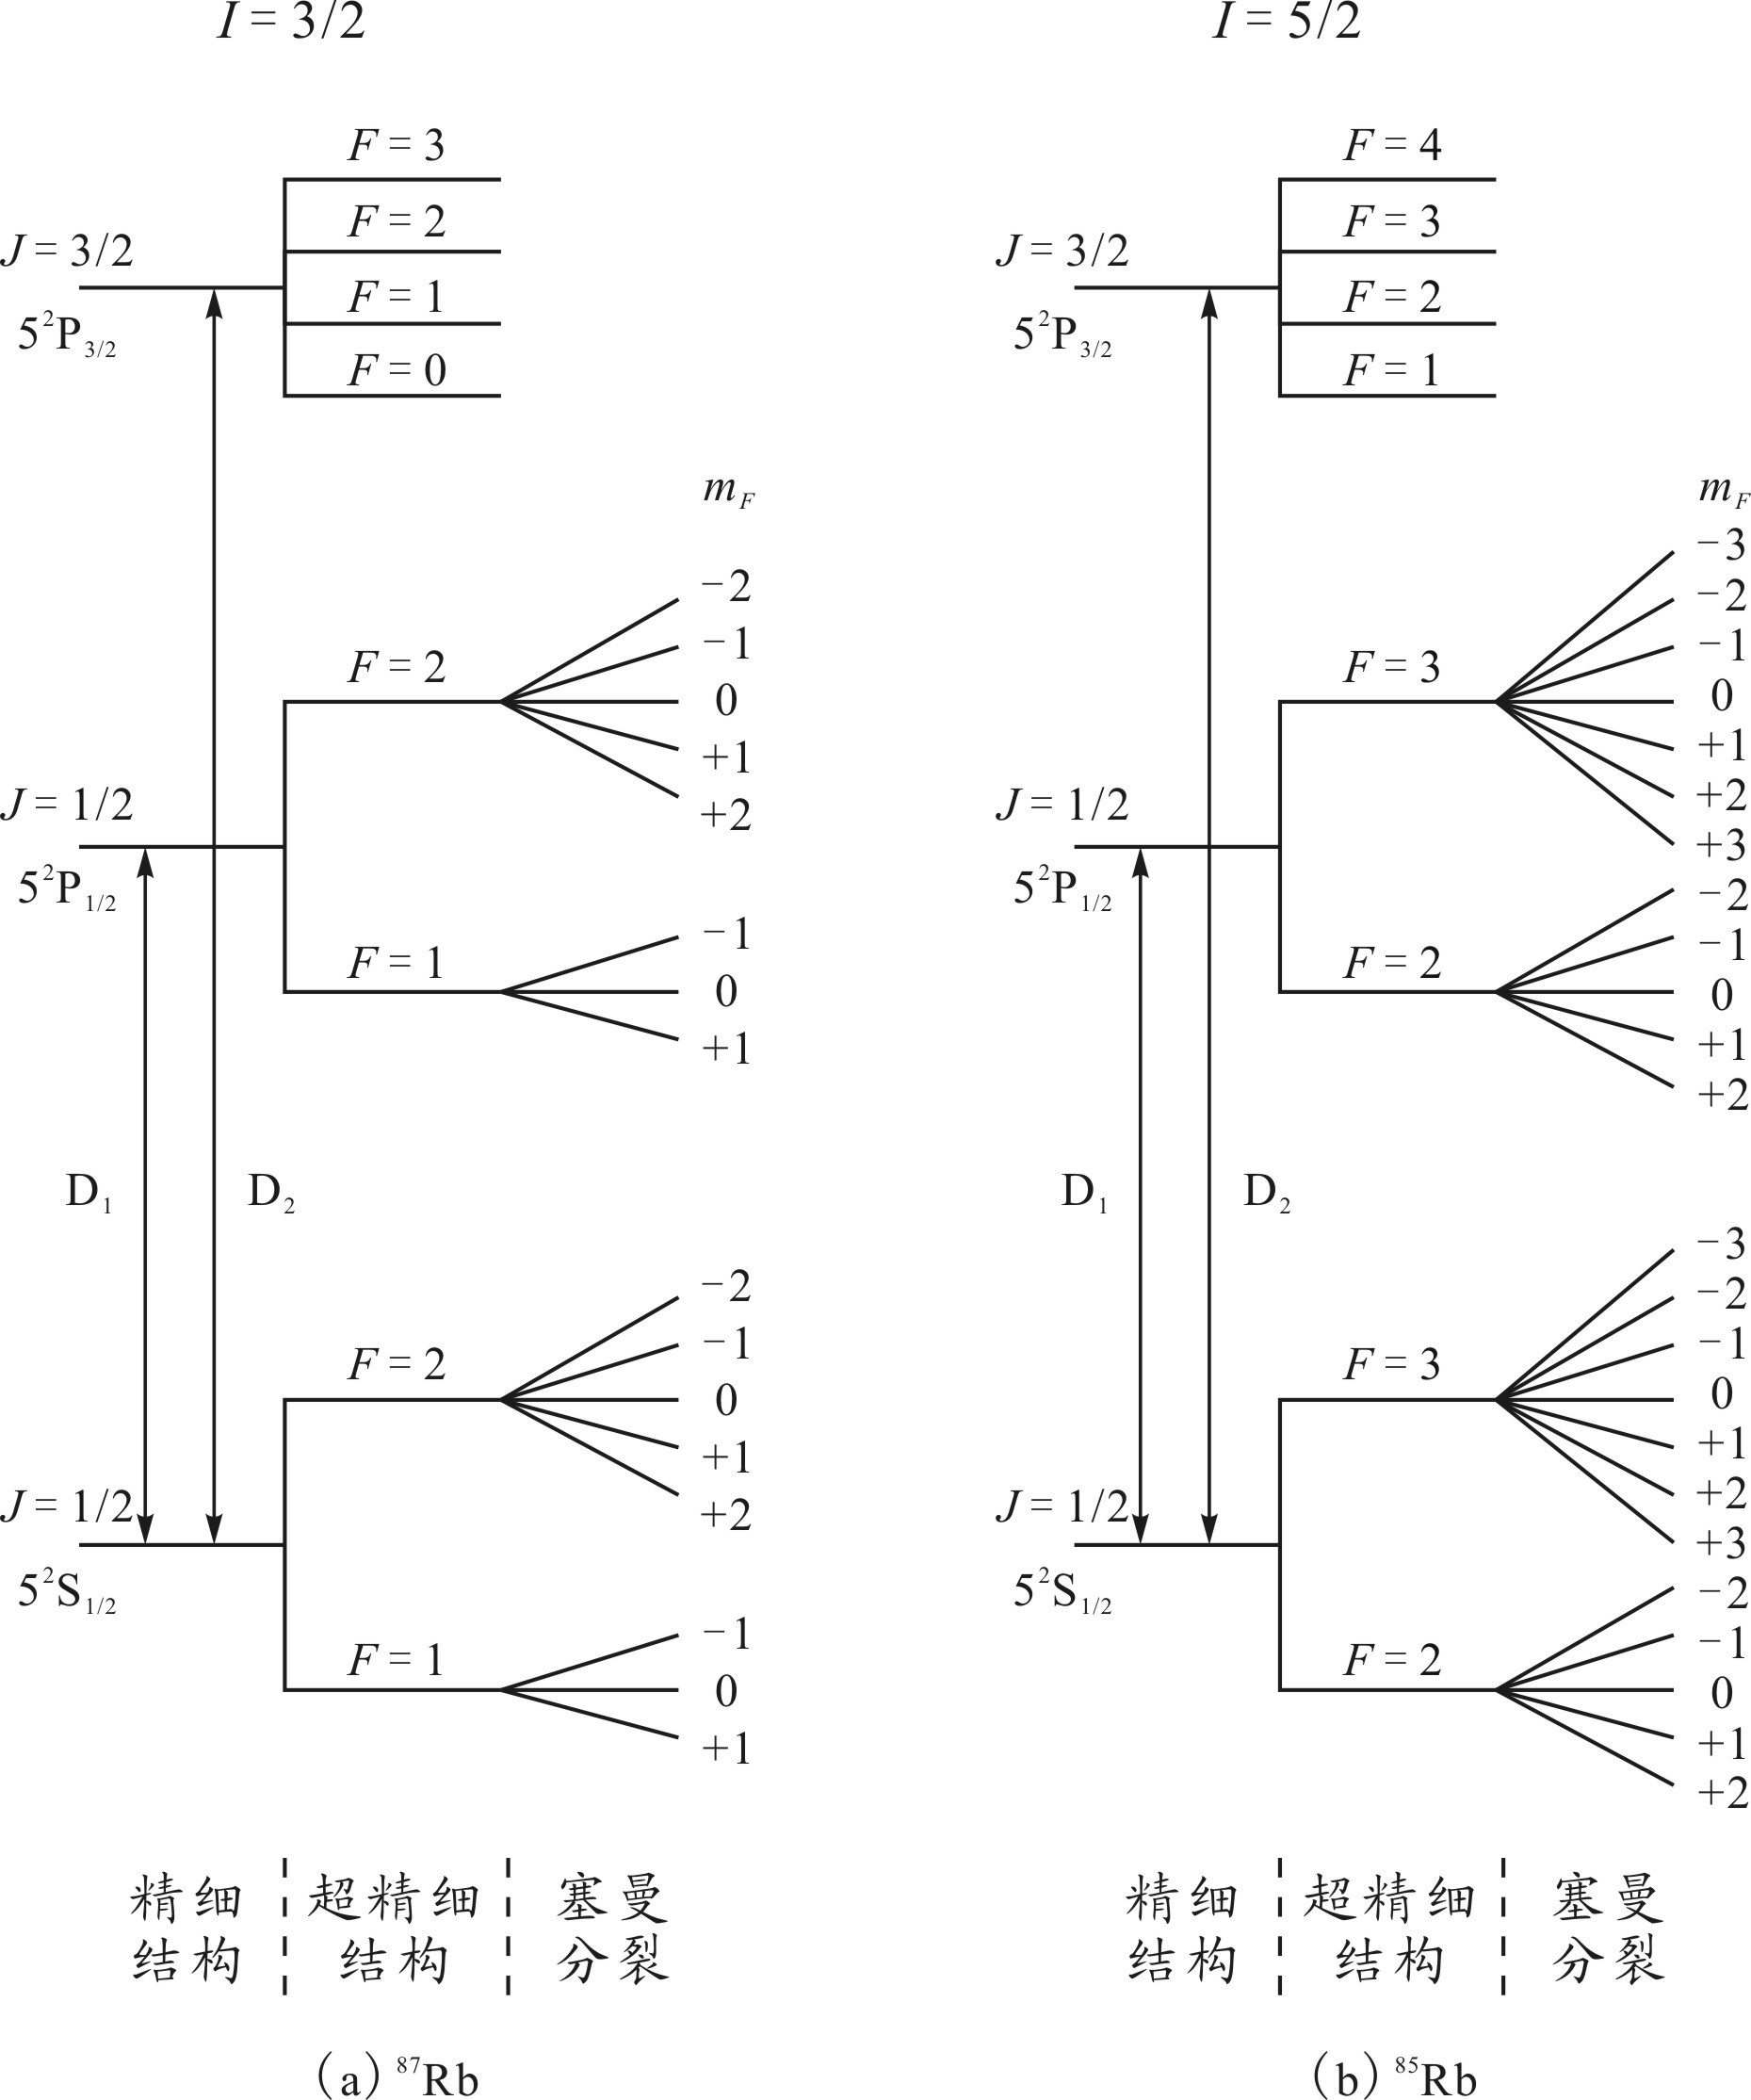
\includegraphics[width=.6\textwidth]{fig2-6-1}
\caption{$^{85}Rb$和$^{87}Rb$基态及最低激发态的能级示意图}
\label{fig2-6-1}
\end{figure} 

\subsection{光抽运产生偏极化}
在热平衡状态下,各能级的粒子数遵从玻尔兹曼分布,能级$E_1$和$E_2$上粒子数之比
\begin{eqnarray} \label{2-6-6}
N_2/N_1=e^{-\Delta E/kT},
\end{eqnarray}
式中$\Delta E=E_2-E_1$为两个能级间的能量差,$N_1$和$N_2$分别为能级$E_1$和$E_2$的原子数,
$k$为玻耳兹曼常数。由于超精细塞曼子能级间的能量差很小,可以近似地认为这些子能级上的粒子数相等。\par
光抽运是建立在光跃迁过程角动量守恒的基础上,通过带偏振光激发原子,是原子能级的粒子布局数发生改变。
由于光波中磁场对电子的作用远小于电场对电子的作用,故光对原子的激发,可以看成是光波的电场部分起作用。
设偏振光的传播方向与外磁场$B$同方向,左旋圆偏振光$\sigma^+$的角动量为$+\hbar$;
右旋园偏振光$\sigma^-$的角动量为$-\hbar$;线偏振 光$\pi$可看成是两个旋转方向相反的园偏振光的叠加,其角动量为零。
\par 
偏振光激发时,光跃迁遵守选择定则
\begin{eqnarray} \label{2-6-7}
\Delta L=\pm 1,\Delta L=0,\pm1,\Delta m_F=\pm1.
\end{eqnarray}
当入$D_1\sigma^+$光作用于$^{87}Rb$时,在$5^2S_{1/2} \to 5^2P_{1/2}$的激发跃迁中,由于$\sigma^+$光子的角动量为+,
只能产生$\Delta m_f=+1$的光跃迁。基态$m_F=+2$子能级上粒子若吸收光子必将跃迁至$m_F=+3$的能态,
由于$5^2P_{1/2}$各子能级最高为$m_F=+2$,因此基态中$m_F=+2$子能级的粒子$D_1\sigma^+$光激发产生跃迁的几率为零。
$D_1\sigma^+$光只能将基态中除$m_F = +2$以外各子能级的原子激发到$5^2P_{1/2}$的相应子能级上,如图~\ref{fig2-6-2}(a)所示。\par
跃迁到$5^2P_{1/2}$上的原子通过自发辐射及无辐射跃迁两种过程,以相等的几率回到基态$5^2S_{1/2}$各个子能级。
如图~\ref{fig2-6-2}(b)所示。这样,经过多次受激$\to$返回,基态$m_F=+2$子能级上的粒子数只增不减,
即基态其他能级上的粒子被抽运到基态$m_F=+2$子能级上,从而达到粒子布居数偏极化的目的。
 \begin{figure}[!htbp]
\centering
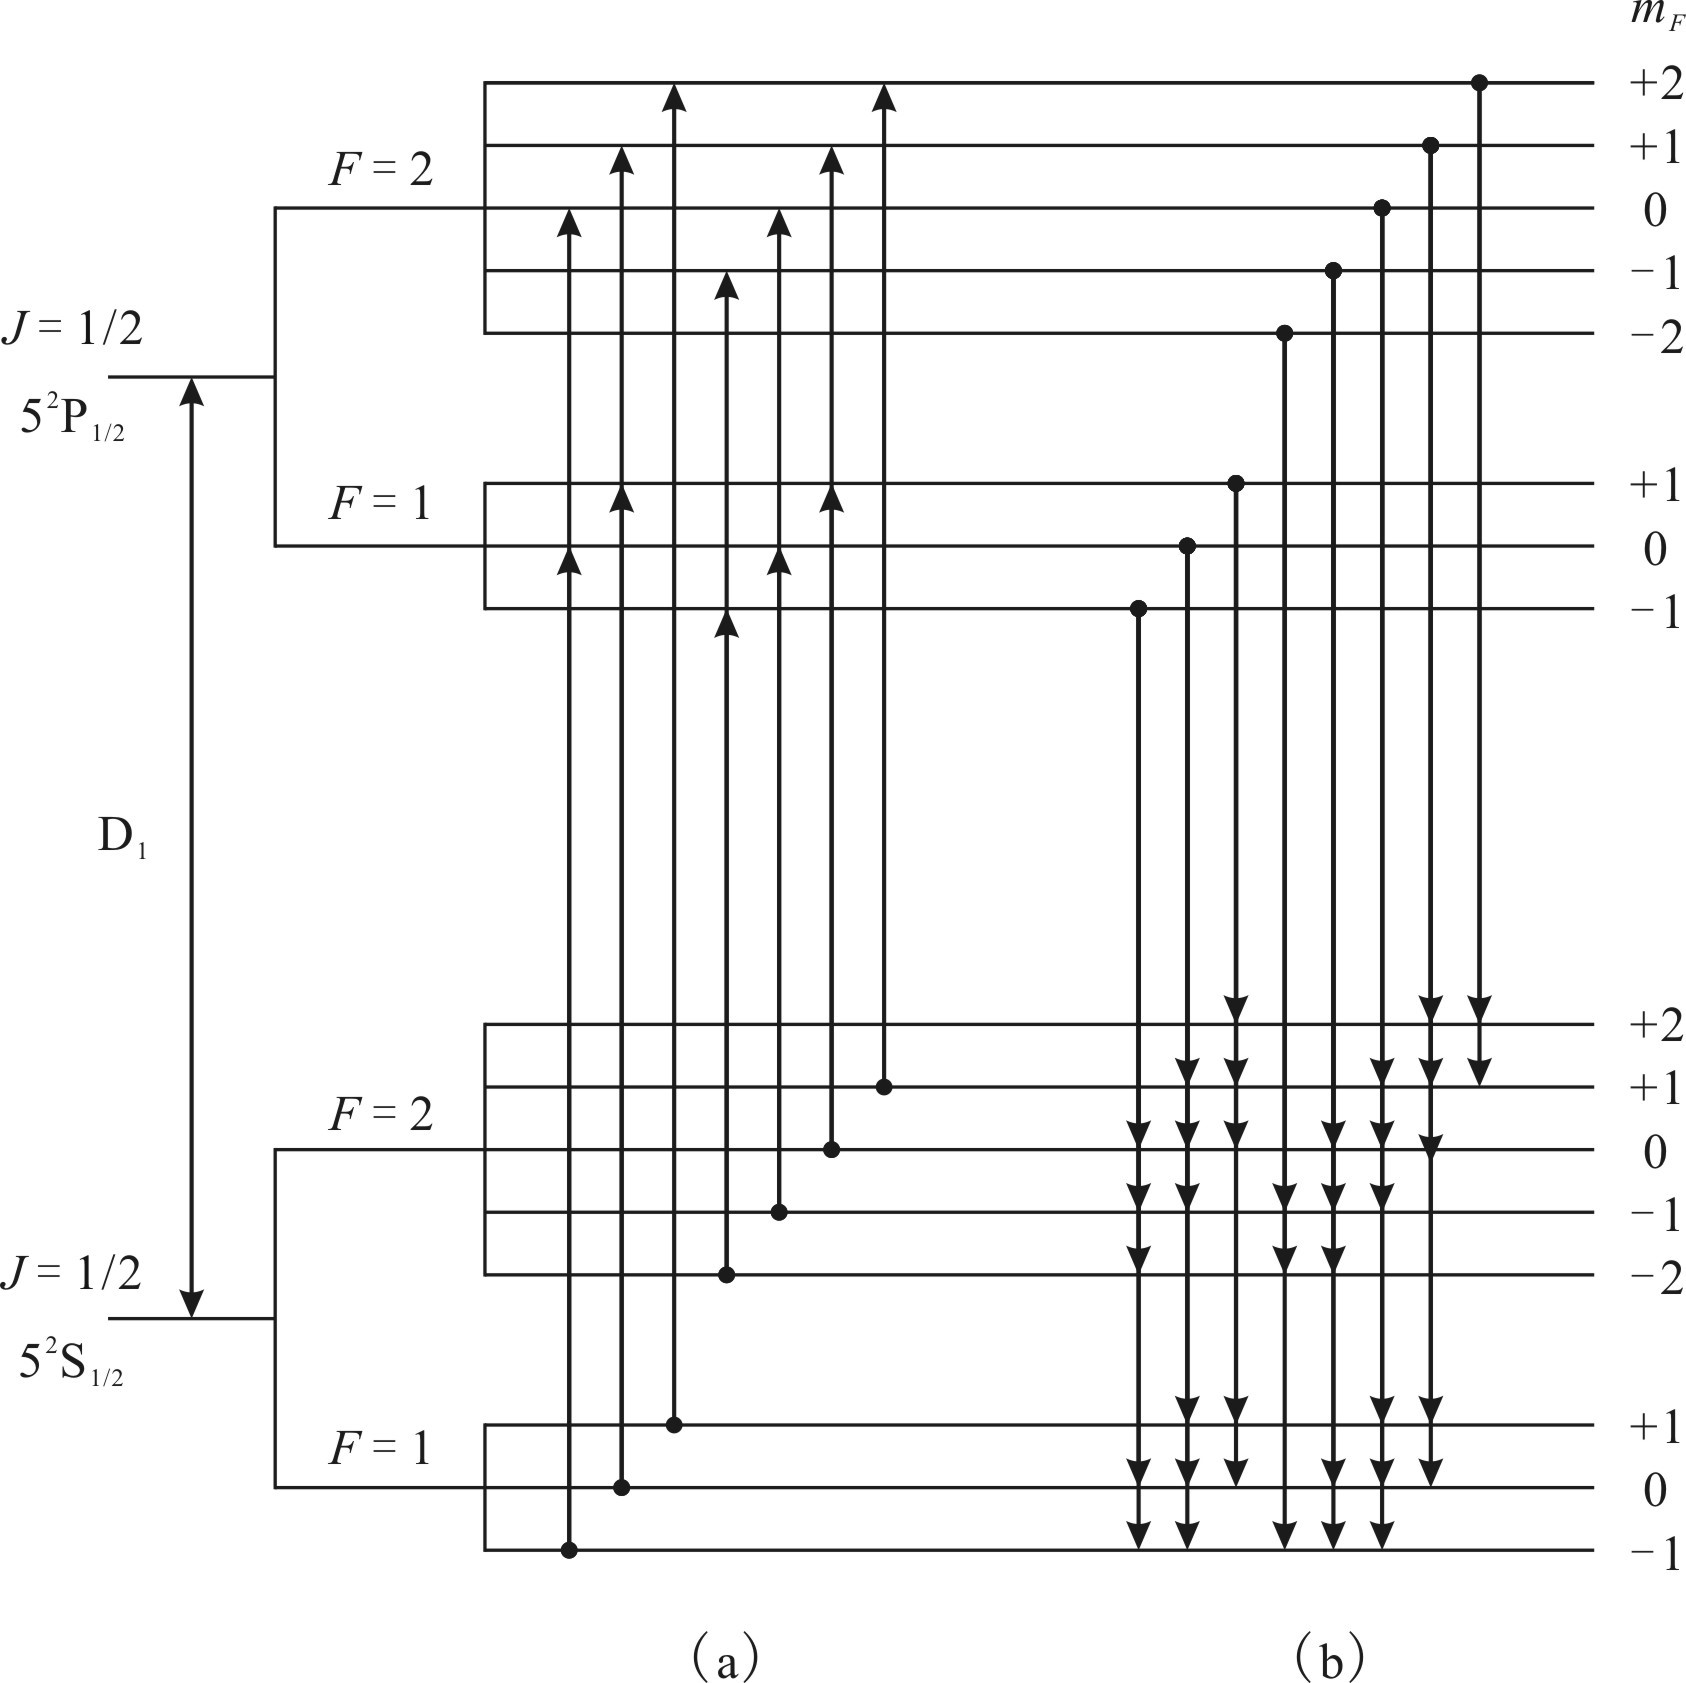
\includegraphics[width=.6\textwidth]{fig2-6-2}
\caption{光抽运过程}
\label{fig2-6-2}
\end{figure} 
\par
同理,若入射光$D_1\sigma^-$作用于$^{87}Rb$时,则大量粒子将被抽运到$m_F=-2$子能级上。若入
射$D_1\pi$光,由于角动量为零不符合$\Delta m_F = \pm 1$选择定则,不能产生受激非平衡分布,从而不能产生光抽运效应。\par
对于$^{85}Rb$,若入$D_1\sigma^+$光作用,粒子将被抽运到$m_F=+3$子能级上;入射$D_1\sigma^-$光时,
粒子将被抽运到$m_F=-3$子能级上;同理,入射$D_1\pi$光不能产生光抽运效应。

\subsection{弛豫过程}
光抽运使原子系统能级分布偏极化而处于非平衡状态,但驰豫过程令系统趋向于平衡分布状态,促使系统趋于平衡的机制可以是原
子之间或原子与周围其它物质的相互作用及能量交换。在实验过程中要保持铷原子布居数有较大的偏极化程度,
有效办法是尽量减少铷原子之间以及铷原子与容器壁的碰撞几率。通常,在铷样品泡内充入氮或氖等惰性气体作为缓冲物质,
其密度比样品泡中铷蒸气的原子密度约大6个数量级,从而有效减少铷原子与容器壁的碰撞机会。由于缓冲气体的磁性很弱,
它们与铷原子碰撞时对铷原子状态的扰动极小,从而能保持铷原子分布的高度偏极化。当然缓冲气体不可能完全抑制弛豫过程,
所以光抽运不可能把基态上的原子全部抽运到特定的子能级上。\par
铷样品泡温度对原子系统的驰豫过程有很大影响。铷样品泡温度升高,铷蒸气的原子密度增加,
铷原子与容器壁之间以及铷原子相互之间的碰撞机会增加,必将导致铷原子能级布居数偏极化减少。若铷样品泡温度太低,
铷蒸气的原子数目太少,则抽运信号幅度很小不便于实验观测。因此,实验将铷样品泡温度控制在$40\sim 50^{\circ}$C间。\par

\subsection{磁共振与光检测}
光抽运使铷原子能级粒子数分布偏极化达到饱和之后,铷蒸气不再吸收入射的圆偏振光,从而使透过铷样品泡的光强增大。
若在垂直产生塞曼分裂的外磁场$B$的方向施加一频率为$\nu$的射频磁场,当$\nu$和$B$之间满足磁共振条件
\begin{eqnarray} \label{2-6-8}
h\nu = g_F\mu_FB
\end{eqnarray}
时,便发生塞曼子能级之间的共振跃迁现象,这种现象称为磁共振。跃迁遵守选择定则
\begin{eqnarray} \label{2-6-9}
\Delta F=0,\Delta m_F=\pm1.
\end{eqnarray}
\par
若入射光$D_1\sigma^+$作用于$^{87}Rb$,由于满足式~\eqref{2-6-8}的射频场使占居$m_F=+2$能级的粒子跃迁至$m_F=+1$能级,
相继又跃迁至$m_F=0,-1,-2$等各子能级上。因此,发生磁共振时,处于$m_F=+2$子能级的粒子数小于饱和状态的原子数,
即磁共振使原子分布的退偏极化。与此同时,$D_1\sigma^+$光的作用又将基态中非$m_F=+2$的原子抽运到$m_F=+2$的子能级上。
磁共振跃迁和光抽运相互竞争与制约将使原子系统达到一个新的动态平衡。\par
$D_1\sigma^+$光作用于$^{87}Rb$时,动态平衡存在于$m_F=-2$与$m_F=-1, 0, 1, 2$子能级之间;
$D_1\sigma^+$作用于$^{85}Rb$,是$m_F=+3$与非$m_F=+3$能级粒子数分布的竞争;$D_1\sigma^+$光作用于$^{85}Rb$,
则是$m_F=-3$与非$m_F=-3$的动态平衡。\par
为了达到满足式~\eqref{2-6-8}的磁共振吸收,通常采用固定外磁场$B$改变射频场频率$\nu$或固定射频场频率$\nu$改变外磁
场$B$两种实验观测技术,前者称为扫频法,后者称为扫场法。\par
由上述分析可知,在偏极化状态下样品对入射光的吸收甚少,特别是当处于饱和状态时,透过铷样品泡的圆偏振光达到恒定;
一旦发生磁共振跃迁,样品对圆偏振光的吸收随之增大,透过样品泡的光强减弱。从而,
只要测量通过铷样品泡透射圆偏振光强的变化即可达到检测磁共振吸收信号的目的。由此可见,
投射到样品的圆偏振光既起抽运作用又可通过透射光强变化检测磁共振信号,即一束光起到了抽运和检测两重作用。\par
由于天然铷样品含有$^{85}Rb$和$^{87}Rb$,从上述分析可知,它们都能被$D_1\sigma^+$或者$D_1\sigma^-$光抽运而产生磁共振吸收,
实验上可以根据它们对应的朗德因子$g_F$不同加以区分。

\section{实验技术方法}
光泵磁共振实验装置由主体单元和辅助设备组成,如图~\ref{fig2-6-3}所示。
\begin{figure}[H]
\centering
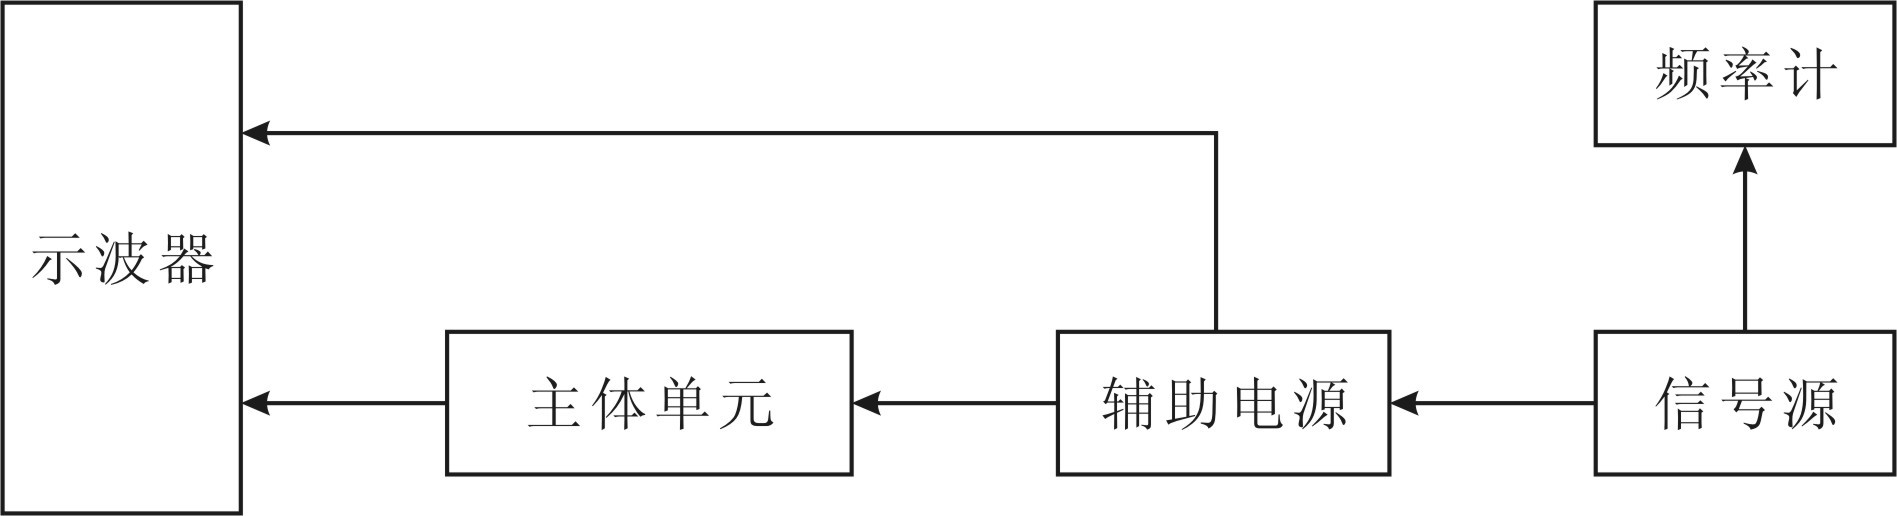
\includegraphics[width=.6\textwidth]{fig2-6-3}
\caption{光泵磁共振实验装置方框图}
\label{fig2-6-3}
\end{figure} 
\par 
主体单元结构如图~\ref{fig2-6-4}所示,各元件的用途说明如下:
\begin{figure}[!htbp]
\centering
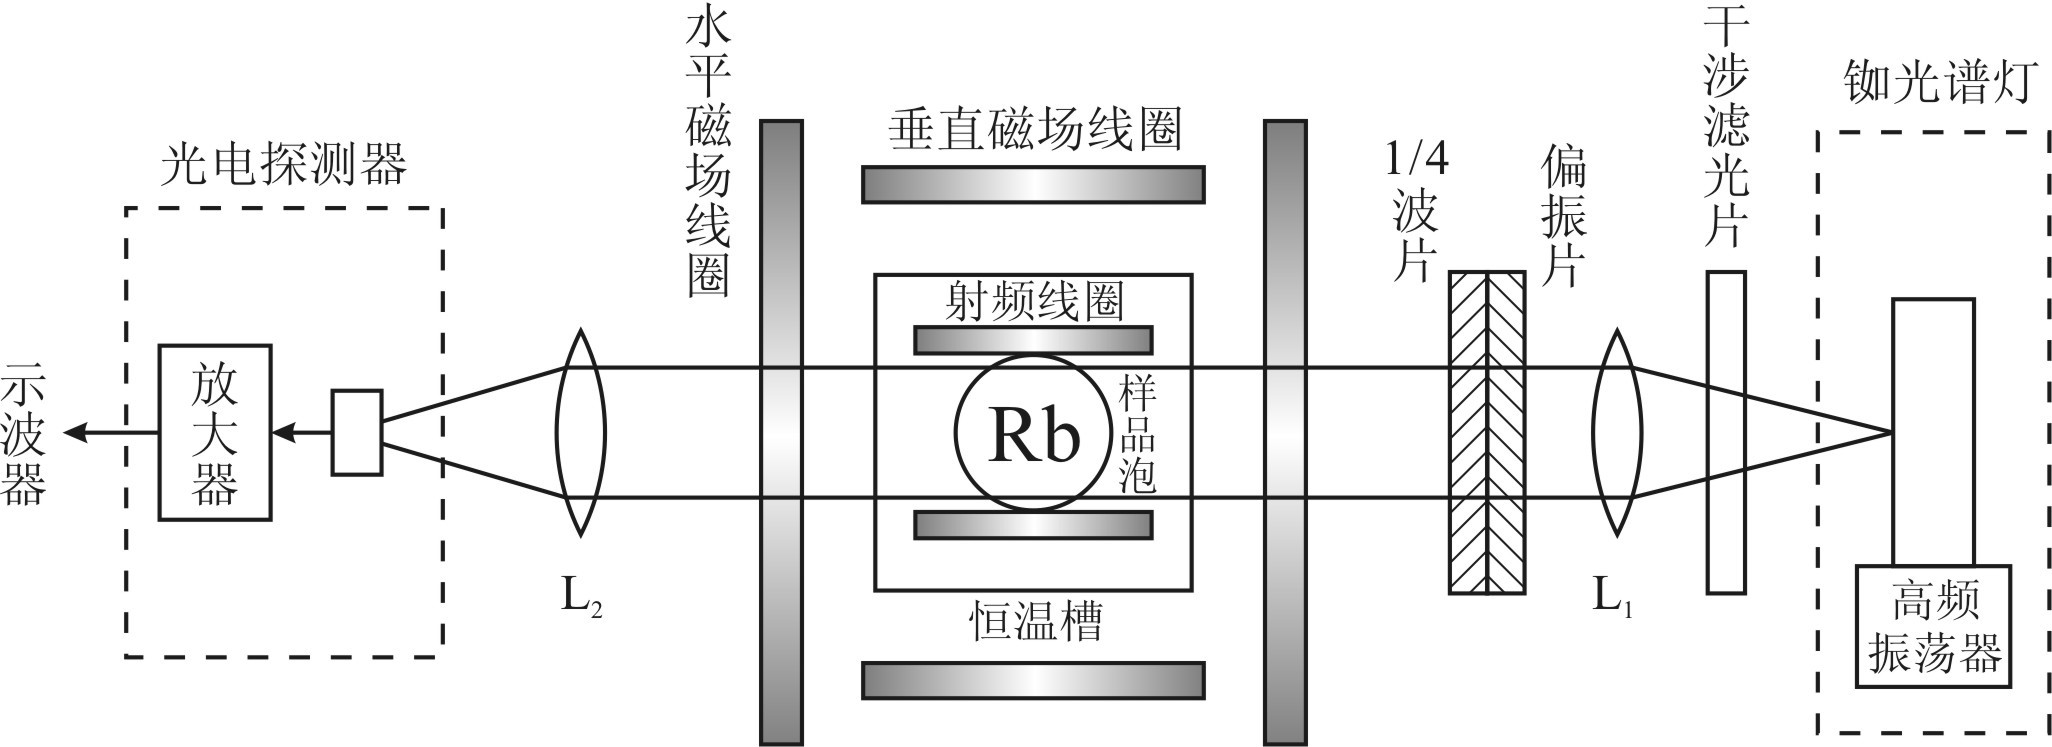
\includegraphics[width=.8\textwidth]{fig2-6-4}
\caption{实验装置主体单元示意图}
\label{fig2-6-4}
\end{figure} 
\begin{enumerate}
\item 抽运光源  主要由高频振荡器(频率约为$55\sim65 MHz$)、控温装置($80\sim90^{\circ}C$)和铷原子光谱灯组成。
铷灯泡在高频电磁场的激励下进行无极放电而发光,产生铷光谱,包括$D_1=7948A$及$D_2=7800A$光谱线。
$D_2$光谱线对光抽运过程有害,出光处装一干涉滤光片,其中心波长为$7948\pm50A$,将不利于光抽运的$D_2$线滤掉。
$D_1$由凸透镜$L_1$变为平行光束,偏振片使得平行光束转为线偏振光,经过1/4波片获得$D_1\sigma ^+$光投射至铷样品泡。
\item样品和磁场  天然成分铷原子和密度约大6个数量级的缓冲气体充在直径为$52mm$的玻璃泡内。在铷样品泡的两侧对称放
置一对射频线圈,为铷原子磁共振跃迁提供射频。铷样品泡和射频线圈均置于圆柱形恒温槽(吸收池)内,
槽内温度为$40\sim 50^{\circ}C$连续可调。\par
吸收池安放在两对亥姆霍兹线圈的中心。一对竖直线圈产生的磁场用以抵消地磁场的竖直分量。另一对水平线圈有两套绕组。
一组在外,为产生水平直流磁场的线圈。另一组在内,为扫场线圈,扫场是在直流磁场上叠加的一个调制磁场(方波或三角波)。
要注意,使铷原子的超精细结构能级发生塞曼分裂的是水平方向的总磁场。\par
各组亥姆霍兹线圈在铷样品泡处所产生的磁场由下式求得
\begin{eqnarray} \label{2-6-10}
B=4.496 \frac{NI}{r},
\end{eqnarray}
式中,$N$为线圈每边匝数,$I$为流经线圈的励磁电流强度(A),r为线圈的有效半径(m),计算得到的磁场$B$的单位是$T$。
产生塞曼分裂的是水平方向的总磁场,包括直流磁场、扫场和地磁场水平分量。
\item光信号检测  透过铷样品泡的光束经焦距为$77 mm$凸透镜$L_2$会聚到光电探测器上,经转化为电信号放大用于实验观测。
\begin{figure}[ht]
\centering
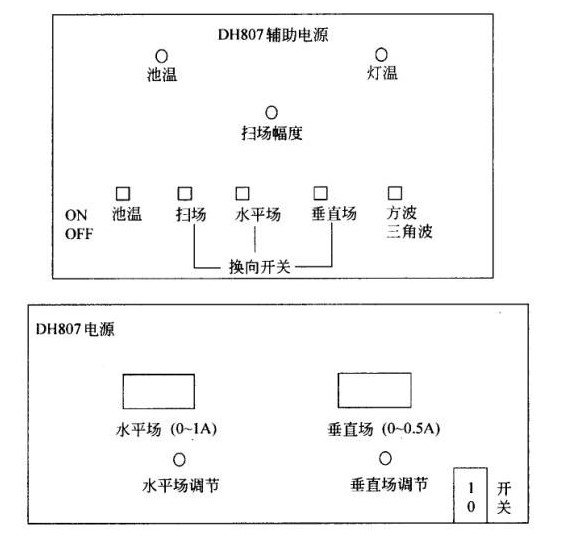
\includegraphics[width=.8\textwidth]{added}
\caption{DH807辅助电源前面板}
\label{fig3.9}
\end{figure}
\item辅助设备  辅助设备包括辅助源、射频信号发生器、数字频率计和(双通道)示波器。示波器通常采用双通道方法:
一个通道观测扫场信号;另一个通道观测光抽运和磁共振信号。
\par
由实验装置方框图可以看到。射频信号是先输入辅助电源,再由24芯电缆将辅助电源与主体装置联接起来。
射频信号发生器($20KHz\sim 1MHz$)可以指示射频信号的频率值,功率大小可以调节。辅助电源上附有测水平线圈与竖直线圈励磁电流的电表,
用以测水平场励磁电流和竖直场励磁电流等值(单位是安培A)。如图~\ref{fig3.9}中有关部分所示。除射频小线圈外,
所有励磁线圈都有一个极性换向开关和调节励磁电流的旋钮,它们装在辅助电源的前面板上。池温(ON,OFF)开关用于给吸收池加热。
当池温和灯温显示灯亮时,说明池温和灯温已到工作温度。方波和三角波开关以及扫场幅度旋钮可用示波器观察它们的功能。
水平场、水平扫场以及垂直场换向开关的功能可由指南针检验。把指南针放在线圈中心位置,观察调节换向开关后指南针的偏转,
从而判断各磁场方向与地磁场水平和垂直分量方向的关系。辅助电源后面板上有射频信号功率输入插孔和扫场信号输出插孔(已接好)。
\end{enumerate}

\section{实验内容与分析}
\subsection{实验系统调节}
\begin{enumerate}
\item 主体单元放置远离电磁场干扰。借助指南针使导轨安放于地磁场水平分量方向上,调节光源、透镜、铷样品泡和光电检测器件使各元件共轴。
\item 确认实验系统各部分连接正确,接通DH807A电源开关,置“池温”按钮于 “ON”位置。开示波器电源,或启动计算机数据采集系统。
\item 预热约20分钟。灯温指示灯亮,铷光谱灯点燃并发出紫红色光;池温指示灯亮,吸收池进入正常工作状态。
\item 调节凸透镜$L_1$位置使出射平行光束作用于铷样品泡上;调节凸透镜$L_2$将平行光束会聚到光电检测器使检测光强最大。
\item调节偏振片和1/4波片与光轴的夹角,结合下一步“光抽运信号观测”使光抽运信号最大,并旋紧锁定环。
\end{enumerate}
以上调节确保实验装置达到最佳状态,在随后的磁共振信号观测中尽可能避免碰触主体单元各个元件,以期获得准确的实验数据。\par
%岱山)在本次实验中步骤(4)和(5)略去。(??????????????????)

\subsection{光抽运信号观测}
采用方波和三角波磁场都能观测光抽运信号,但方波能较快的通过零点建立正向或反向磁场,故观测光抽运信号时常使用方波磁场,
即本实验选用的方波扫场。刚加磁场的一瞬间,铷原子基态各塞曼子能级上的粒子数接近热平衡分布,可认为各子能级上的粒子数近似相等,
对于$^{87}Rb$来说,约有7/8的粒子可吸收$D_1\sigma^+$光,因此这一瞬间对光的吸收最强。随着粒子逐渐被抽运到$m_F=+2$子能级上,
能吸收$D_1\sigma^+$光的粒子数减少而对光的吸收减少,透过铷样品泡的光强逐渐增强。当抽运到$m_F=+2$子能级上的粒子数达到饱和时,
透过铷样品泡的光强达最大而不再变化。直到磁场过零(指水平方向的总磁场过零)并反向时,塞曼子能级跟随着发生简并随即再分裂。
当能级简并时,塞曼子能级消失而使铷原子失去了偏极化。但当磁场反向重新分裂后各子能级上的粒子数近乎相等,
此时对(相当于)$D_1\sigma^-$光的吸收达到最大(粒子被抽运到$m_F=+2$的子能级上)。上述过程周而复始,
从而可在示波器上观测到周期性光抽运信号。\par
实验中用于观测光抽运信号的方波或三角波磁场较弱,地磁场足以产生较大的影响。通过采用不同波形扫场,
分别观测水平线圈磁场和竖直线圈磁场以及改变他们的励磁电流大小和方向对光抽运信号的影响。\par
当竖直线圈产生的磁场完全抵消地磁场垂直分量时,光抽运信号达到最大值。保持这一状态的竖直线圈励磁电流大小和方向,
以便更好的进行磁共振信号观测。

\subsection{光抽运的磁场关系(半定量分析,选做)}
改变竖直线圈励磁电流大小和方向,光测并详细记录光抽运信号的变化,研究光抽运信号(峰面积)与垂直磁场的关系。
使合成磁场垂直分量为零(光抽运信号达到最大),改变水平线圈励磁电流大小和方向,观测并详细记录光抽运信号的变化,研究光抽运信号
(峰面积)与水平磁场的关系。基于物理基础原理,对实验数据进行拟合分析,并对上述物理现象作出合理解释。

\subsection{磁共振信号观测}
光抽运信号反映了铷原子基态$5^2S_{1/2}$和最低激发态$5^2P_{1/2}$超精细结构塞曼子能级之间的光学跃迁,
可观测的光抽运吸收源于周期性变化且穿越零点的磁场。在磁场正向零点反向的过程中,塞曼子能级表现为分裂$\to$简并$\to$再分裂,
而粒子布居数经历了极化$\to$退极化$\to$再极化的变化。同理,可观测的磁共振吸收信号源于粒子布居数极化与退极化的物理变化。
与纯光抽运过程不同,磁共振过程的退极化是由满足于式~\eqref{2-6-8}的射频跃迁来实现,这是区分两种物理现象的实验判据。\par
对于选定的射频场频率$\nu$,改变外磁场$B$ 使满足式~\eqref{2-6-8},可以获得$^{85}Rb$和$^{87}Rb$的磁共振信号;
对于设定的外磁场$B$,改变射频场频率$\nu$使满足式~\eqref{2-6-8},同样可以获得$^{85}Rb$和$^{87}Rb$的磁共振信号。
为便于实验操作,建议采用前一种方法(即扫场法),且选用三角波扫场进行实验观测。确认合成磁场垂直分量为零(光抽运信号达到最大),
调节适量的射频场幅度,选择适当射频场频率$(300\sim 400MHZ)$和信号功率输出,
详细观测$^{85}Rb$和$^{87}Rb$的磁共振信号随水平磁场强度和方向的变化。在磁共振点附近选定水平磁场强度,
观察记录$^{85}Rb$和$^{87}Rb$ 的磁共振信号随三角波扫场的波谷、波峰及腰部的实验条件,从而选择便于观测的实验测量参考点,
进行郎德因子$g_F$分析。

\subsection{测量朗德因子$g_F$}
通过测量磁共振对应的射频场频率$\nu$和外磁场$B$ ,由式~\eqref{2-6-8}可以确定$g_F$值。事实上,在实验中外磁场$B$包括了水平
禾姆霍兹线圈产生的磁场$B_P$、扫场$B_s$以及地磁场水平分量$B_{\parallel}$,即
\begin{eqnarray} \label{2-6-11}
B=B_P+B_S+B_{\parallel}.
\end{eqnarray}
\par
磁场$B_P$可通过测量水平禾姆霍兹线圈励磁电流$I$,并由式~\eqref{2-6-10}求得。通常,在实验测量中采用固定的扫场$B_S$
(大小和方向),而地磁场水平分量$B_{\parallel}$ 可认为是恒定值,从而$(B_S+B_{\parallel})$为常数。在扫场法中,
对于每预设频率$\nu$的射频场,通过测量磁共振对应的正向和反向水平磁场的平均值,即可求得朗德因子$g_F$。显然,
在$|B_P|>|B_S+B_{\parallel}|$情形,上述方法确实简单可行。但是当$|B_P|<|B_S+B_{\parallel}|$时可能出现对作用于样品总
磁场方向判断错误而得不出正确的实验结果。尽管已有多篇文章对这一问题进行深入探讨分析,并提出多种实验测量改进方法,
但我们必须认识到:平均法只是一种纯数学方法,它缺乏实验数据分析的物理依据,这是导致出现不合理试验结果的根本原因。\par
当偏振光的传播方向与外磁场$B$同向,实验使用的是左旋圆偏振光$D_1\sigma$起$\sigma^+$作用,它将$^{85}Rb$和$^{87}Rb$粒
子分别抽运到$m_F=+3$和$m_F=+2$能级;当偏振光的传播方向与外磁场$B$逆向,实验用偏振光$D_1\sigma$起$\sigma^-$作用而将
$^{85}Rb$和$^{87}Rb$粒子分别抽运到$m_F=-3$和$m_F=-2$能级。显然这是两种不同的物理过程,合理的数据分析必须基于相同物
理过程的实验测量。由式~\eqref{2-6-8}和~\eqref{2-6-11},可得
\begin{eqnarray} \label{2-6-12}
h\nu=g_F\mu_BB_P+g_F\mu_B(B_S+B_{\parallel}).
\end{eqnarray}
%上式到底是$\mu_F$还是$\mu_B$?????
\par
在实验过程中地磁水平分量$B_{\parallel}$和扫场大小与方向保持恒定,若在实验测量中吸收峰定位方法保持一致,
式~\eqref{2-6-12}中第二项 必为常数。因此,同一磁共振信号对应的一组$(\nu,B)$为线性关系。通过线性拟合,
可以获得$^{85}Rb$和$^{87}Rb$分析在$\sigma^+$和$\sigma^-$作用时的实验结果。

\section{实验数据分析}


\section{思考与讨论}
\begin{enumerate}
\item 实验过程中如何区分光抽运与磁共振信号?如何区分$^{85}Rb$和$^{87}Rb$磁共振信号?\par 
这两种信号从图形上看均是向下凹陷的循环的尖锐峰;因而直接通过形貌特征很难判别;而由于实验的铷蒸汽中同时
有$^{85}Rb$和$^{87}Rb$两种同位素参与共振过程,因而可以通过共振信号曲线能够劈裂出双峰的特征来分别。具
体来说就是通过调节射频场的频率,如果看到单峰图形能够劈开变为双峰图形的,是磁共振信号,否则看到的是光抽
运信号。或者从操作上分析,也可以依据抽运信号与射频信号无关,但磁共振吸收需要满足磁共振条件
\begin{eqnarray} 
h\nu = g_F\mu_FB.
\end{eqnarray}
光抽运吸收源于周期性变化且穿越零点的磁场,而磁共振吸收源于粒子数极化与退极化,故可调节射频场频率来判断。\par
实验中通过操作发现,要从一个单独的磁共振信号中判断这是$^{85}Rb$或$^{87}Rb$的信号时很困难的,但是当在
一个连续变化的频率范围内出现两个或者更多的共振信号时,便可以通过两个同位素的共振频率的比例关系来判断。\par 
\item 为什么实验测量中同一物理过程采用扫场不变且相同的磁共振信号定位方法可以满足$(\nu,B_P)$的线性关系?\par 
根据原理部分的式~\eqref{2-6-12},即
\begin{eqnarray} 
h\nu=g_F\mu_BB_P+g_F\mu_B(B_S+B_{\parallel}),
\end{eqnarray}
可得$B_S+B_{\parallel}$固定时,$(\nu,B_P)$满足线性关系。
\item  采用不同的磁共振信号定位方法影响朗德因子的实验结果吗?\par 
不影响。朗德因子是粒子本身的特性,不同的磁共振信号会造成$B_S+B_{\parallel}$变化,即截距变化,但不会影
响到直线的斜率,即不影响朗德因子的测定。
\item  如何理解曲线拟合方法在$|B_P|<|B_S+B_{\parallel}|$情形的合理性?曲线拟合所求得的截距的物理意义是什么?\par 
在$|B_P|<|B_S+B_{\parallel}|$情形下,三角波扫场强度比较大,覆盖了光抽运信号和$^{85}Rb$或$^{87}Rb$
共振吸收信号所需的磁场范围,并出现截距差异。这个差异反映了光磁共振吸收处$B_S$的作用量不同,即所得截距
$-(B_S+B_{\parallel})$,在$B_S$大小可忽略时,截距的物理意义是地磁场的水平分量大小。
\item  磁场垂直分量不为零,实验结果如何?\par 
磁场垂直分量不为零时,总外加磁场不水平,此时光抽运信号不能达到最大值。而磁场完全水平时,光抽运信号最明
显。根据式~\eqref{2-6-12},其中的$B_{\parallel}$变成垂直与水平分量之和,计算带入数据会偏小,推算的
朗德因子会偏大。
\item  如何测量实验所在处的地磁场?请拟定实验步骤和结果分析方法。\par
可以分别求出水平和垂直分量。首先测量地磁场的垂直分量。由于光抽运信号最明显时,附加垂直磁场完全抵消地
磁场垂直分量,我们可以这样求得地磁场垂直分量。\par 
再测量地磁场水平分量。调节三角波扫场方向,在其与地磁场水平分量分别为同向和反向时测量$(\nu,B_P)$的线性
关系,并根据式~\eqref{2-6-12},即
\begin{eqnarray} 
h\nu=g_F\mu_BB_P+g_F\mu_B(B_S+B_{\parallel}),
\end{eqnarray}
求得
\begin{eqnarray} 
B_{\parallel}=\frac{h(\nu_1+\nu_2)}{2 g_F\mu_B}.
\end{eqnarray}
\end{enumerate}




%\medskip
%\renewcommand{\refname}{参考文献}
%\begin{thebibliography}{99}
%\bibitem{wiki}Franck–Hertz experiment. Wikipedia[DB/OL]. \url{http://en.wikipedia.org/wiki/Franck%E2%80%93Hertz_experiment}.
%\bibitem{ref01}蔡文. 可拓论及其应用[J]. 科学通报, (1999),44(7), 673-682.
%\bibitem{data}Hg (all spectra). NIST Atomic Spectra Database Lines Data[DB/OL]. \url{http://physics.nist.gov/cgi-bin/ASD/lines1.pl}.
%\bibitem{ref03}杨福家. 原子物理学[M]. 高等教育出版社,北京. 2008.
%\bibitem{reffh}Rapior, G.; Senstock, K.; Baev, V.. New features of the Franck–Hertz experiment[J]. Amer. J. Phys. (2006), 74: 423–428.
%\bibitem{ref03}Warren J. Smith. Modern Optical Engineering[M]. McGraw-Hill Education,New York. 2007.
%\bibitem{ref04}曹炳元. 物元分析法及其在投资决策中的应用[C]. 中国第二次物元分析学术讨论会论文选. 广州, 1986.
%\end{thebibliography}
\end{CJK*}
%\begin{CJK*}{UTF8}{gbsn}
%\newpage
%\renewcommand{\appendixname}{附录}
%%\appendix
%\begin{appendices}
%  \renewcommand\thetable{\thesection\arabic{table}}
%  \renewcommand\thefigure{\thesection\arabic{figure}}
%  \section{电子自旋共振实验}
%  日期:2015.10.13 \hfill{} 室温:25.0$^\circ C$ \hfill{}湿度:75.0\% \hfill{}实验人:胡乃超 \ 金谷柳新
%  \section{实验过程记录} \label{app:foobar}
%
%\end{appendices}
%\end{CJK*}
\end{spacing}
\end{document}
